\documentclass[12pt]{article}

\usepackage{setspace}
\usepackage{amsmath,amssymb}
\usepackage{amsfonts}
\usepackage{graphicx}
\usepackage[pdftex,bookmarks=true,bookmarksopen=false,bookmarksnumbered=true,colorlinks=true,linkcolor=black]{hyperref}
\usepackage[utf8]{inputenc}
\usepackage{float}
\usepackage{pdfpages}

\usepackage[brazil]{babel}
% \usepackage[alf]{abntex2cite}	% Citações padrão ABNT

%\usepackage{pstricks}%, egameps}

%\setlength{\textwidth}{17.2cm}
% \setlength{\textheight}{23cm}
%\addtolength{\oddsidemargin}{-22mm} 
%\addtolength{\topmargin}{-15mm} \addtolength{\evensidemargin}{-15mm}
%\setlength{\parskip}{1mm}
%\setlength{\baselineskip}{500mm}

\usepackage[style=abnt]{biblatex}
\addbibresource{refs.bib}  

\newtheorem{theorem}{Theorem}[section]
\newtheorem{assumption}{Assumption}
\newtheorem{acknowledgment}{Acknowledgment}
\newtheorem{algorithm}{Algorithm}
\newtheorem{axiom}{Axiom}
\newtheorem{case}{Case}
\newtheorem{claim}{Claim}
\newtheorem{conclusion}{Conclusion} 
\newtheorem{condition}{Condition}
\newtheorem{conjecture}{Conjecture}
\newtheorem{corollary}{Corollary}[section]
\newtheorem{criterion}{Criterion}
\newtheorem{defn}{Definition}[section]

\newtheorem{example}{Example}[section]
\newtheorem{exercise}{Exercise}
\newtheorem{lemma}{Lemma}[section]
\newtheorem{notation}{Notation}
\newtheorem{problem}{Problem}
\newtheorem{proposition}{Proposition}[section]
\newtheorem{remark}{Remark}
\newtheorem{solution}{Solution}
\newtheorem{summary}{Summary}
\newenvironment{proof}[1][Proof]{\textbf{#1.} }{\rule{0.5em}{0.5em}}



\begin{document}

\begin{titlepage}
\begin{center}
\textbf{\LARGE Fundação Getulio Vargas}\\ 
\textbf{\LARGE Escola de Matemática Aplicada}\\
\textbf{\LARGE Curso de Graduação em Matemática Aplicada}

\par
\vspace{170pt}
\textbf{\Large Título da dissertação}\\
\vspace{80pt}
\textbf{\Large Emanuel Bissiatti de Almeida}\\
\end{center}

\par
\vfill
\begin{center}
{{\normalsize Rio de Janeiro - Brasil}\\
{\normalsize \the\year}}
\end{center}
\end{titlepage}

\thispagestyle{empty}

\newpage
\begin{center}
\textbf{\LARGE Fundação Getulio Vargas}\\ 
\textbf{\LARGE Escola de Matemática Aplicada}\\
\textbf{\LARGE Curso de Graduação em Matemática Aplicada}

\par
\vspace{100pt}
\textbf{\Large Título da dissertação}


\par
\vspace{65pt}
``\textbf{Declaro ser o único autor do presente projeto de
monografia que refere-se ao plano de trabalho a ser executado para continuidade da monografia e ressalto que não recorri a qualquer forma de colaboração ou auxílio de terceiros para realizá-lo a não ser nos casos e para os fins autorizados pelo professor orientador.}''
\end{center}

\par
\vspace{65pt}
\begin{center}


\hrulefill

\vspace{5pt}
\textbf{\Large Nome}
\end{center}

\par
\vfill
\begin{center}
{{\normalsize Rio de Janeiro - Brasil}\\
{\normalsize \the\year}}
\end{center}

\thispagestyle{empty}

\newpage
\begin{center}
\textbf{\LARGE Fundação Getulio Vargas}\\ 
\textbf{\LARGE Escola de Matemática Aplicada}\\
\textbf{\LARGE Curso de Graduação em Matemática Aplicada}

\par
\vspace{100pt}
\textbf{\Large Título da dissertação}


\par
\vspace{65pt}

``\textbf{Projeto de Monografia apresentado à Escola de Matemática Aplicada como requisito parcial para continuidade ao trabalho de monografia.}''
\end{center}

\par
\vspace{65pt}
\begin{center}

\textbf{Aprovado em } \makebox[30pt]{\hrulefill}\textbf{ de }\makebox[120pt]{\hrulefill}\textbf{ de }\makebox[50pt]{\hrulefill}
\\
\vspace{5pt}
\textbf{Grau atribuído ao Projeto de Monografia:} \makebox[30pt]{\hrulefill}\\
\end{center}


\par
\vspace{40pt}
\begin{center}

\hrulefill

\vspace{5pt}
\textbf{Professor Orientador: }\\
\textbf{Escola de Matemática Aplicada}\\
\textbf{Fundação Getúlio Vargas}
\end{center}

\thispagestyle{empty}


% \newpage
% \tableofcontents
% \thispagestyle{empty}

% \newpage
% \section{Introdução}

% introdução...

% \newpage
% \section{Objetivo Final}

% \subsection{xx}

% referencial teórico... \footnote{Ver xx}.

% \subsubsection{yy}

% \newpage
% \subsection{xx}

% xx

\newpage

\section{Introdução}

O acervo de fotografias históricas ImagineRio \cite{imagineRio}, ajuda a visualizar a evolução da cidade do Rio de Janeiro ao longo do tempo. Entretanto, esse retrato da cidade é limitado: as fotografias são escassas, um mesmo edifício possui poucas amostras de fotografias em um mesmo período de tempo e as fotografias não são apenas uma projeção bidimensional da realidade no sensor da câmera \cite{Hartley2004}. O trabalho do Tomás Ferranti \cite{Ferranti2021} apresenta uma ferramenta para que dado uma fotografia de um edifício e a seleção manual das arestas que compõem esse edifício classificadas por direção, seja possível reconstruir tridimensionalmente a fachada desse edifício. Esse trabalho busca automatizar este processo, dado apenas uma imagem de um edifício, por meio de técnicas de visão computacional e aprendizado profundo de máquina seja possível selecionar automaticamente as arestas que compõem esse edifício e classificá-las por direção. Por fim, será proposto uma integrar essa ferramenta ao trabalho do Tomás Ferranti \cite{Ferranti2021} para que seja possível reconstruir as fachadas de um edifício a partir de uma única fotografia.


Para resolver esse problema, esse trabalho computacional foi subdividido em três problemas menores em que cada problema depende da solução do problema anterior. A \textbf{primeira etapa} corresponde a técnicas de detecção de arestas em imagens, na qual o objetivo é classificar cada pixel da imagem em aresta ou não aresta. A \textbf{segunda etapa} corresponde às técnicas de detecção de segmentos de retas, na qual o objetivo é identificar as equações dos segmentos de retas que compõem as arestas da imagem. Por fim, a \textbf{terceira etapa} corresponde às técnicas de classificação de segmentos de retas, na qual o objetivo é usar as propriedades matemáticas das equações das retas e classifica-las de acordo com o ponto de fuga correspondente.

Por hipótese, a solução proposta nesse trabalho considera que os ângulos entre as faces do edifícios são aproximadamente retos e que suas arestas pertencem a uma reta em 3 dimensões. Essa hipótese é razoável, pois, a maioria das construções possuem faces aproximadamente retas e suas arestas pertencem a uma reta em 3 dimensões. Entretanto, essa hipótese não é válida para todos os edifícios, pois, existem alguns edifícios como o Museu de Arte Contemporânea de Niterói, planejado pelo arquiteto Oscar Niemeyer, que possuem faces curvas. O artigo \cite{Ferranti2021} também carrega essas hipóteses, sendo assim, a solução do presente artigo, que é um complemento ao trabalho do Tomás, também leva essas hipóteses em consideração.


As três próximas seções desse trabalho discutirão as técnicas utilizadas para resolver cada um dos problemas propostos: a detecção de arestas, a detecção de segmentos de retas e a classificação de segmentos de retas. A seção INTEGRAÇÂO será dedicada a integrar a solução proposta com a ferramenta desenvolvida pelo Tomás Ferranti. Por fim, a seção CONCLUSÃO apresentará as conclusões desse trabalho e a avaliação dos resultados obtidos.

\section{Detecção de arestas}

A detecção de arestas é um problema clássico de processamento de imagens, onde o objetivo é identificar os limites de objetos contidos em uma imagem. Em especial, esse trabalho busca identificar as arestas que delimitam as faces de edifícios, que em geral são linhas retas. 

\subsection{Algoritmos clássicos}

Os algoritmos clássicos de detecção de arestas são baseados na aplicação de filtros em uma imagem que identificam mudanças bruscas de intensidade. Observe que a imagem de uma aresta é uma região onde a intensidade da imagem muda bruscamente, sendo assim, os algoritmos de detecção de arestas são baseados em filtros que identificam essas mudanças de intensidade por meio de derivadas da intensidade da imagem \cite{shrivakshan2012comparison}. A figura \ref{fig:sobel}, mostra a fotografia do edifício da biblioteca nacional e o resultado da aplicação do algoritmo de Sobel e do algoritmo de Canny.

\begin{figure}[H]
\centering
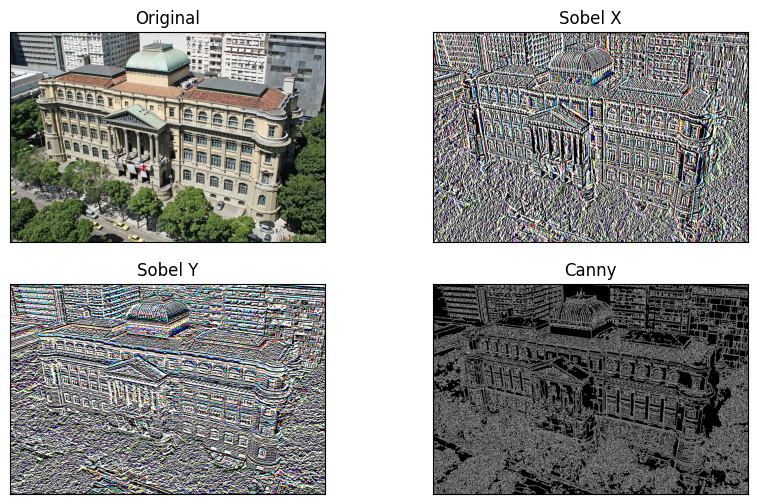
\includegraphics[scale=0.70]{sobel.png}
\caption{Imagem original e resultado do algoritmo de Sobel.}
\label{fig:sobel}
\end{figure}

O algoritmo de Sobel é um filtro convolucional que calcula a magnitude do gradiente da intensidade da imagem. O algoritmo de Canny é um algoritmo mais sofisticado que utiliza o algoritmo de Sobel para calcular a magnitude do gradiente da intensidade da imagem e aplica uma série de filtros para remover ruídos e destacar as arestas da imagem. Em geral o algoritmo de Canny apresenta melhores resultados que o algoritmo de Sobel, porém, o algoritmo de Canny é mais custoso computacionalmente, apesar disso, o custo computacional não é está sendo considerado nesse trabalho.

Em análise, ambos os algoritmos não apresentam resultados satisfatórios para essa aplicação. O algoritmo de Sobel apresenta muitos ruídos e o algoritmo de Canny apresenta muitas arestas que não são relevantes para a aplicação. Essa aplicação busca encontrar as arestas que delimitam as faces de edifícios, entretanto, esses algoritmos detectam todas as arestas da imagem, incluindo as que compõem a textura da parede dos edifícios e as janelas. 

Uma abordagem para resolver esse problema seria utilizar um desses algoritmos e depois aplicar um modelo que seleciona o subconjunto de arestas ótimas para a aplicação, ou seja, do conjunto de arestas dado pelos algoritmos, selecionar apenas aquelas que delimitam os prédios por meio de aprendizado de máquina. Entretanto, essa abordagem não é eficiente, pois, as técnicas de aprendizado de máquina precisa de um conjunto de treinamento para aprender a selecionar as arestas ótimas, e para obter esse conjunto de treinamento é necessário selecionar manualmente as arestas ótimas. Existem alguns conjuntos de que já foram selecionados manualmente, como o banco de dados \cite[Nyu Dataset]{nyu_depth_v2} que realiza uma ótima segmentação de objetos em uma imagem. Porém, para trabalhar com modelos de aprendizado de máquina em imagens é necessário um grande conjunto de dados para treinamento e um grande poder computacional para processar esses dados a qual não está disponível para a realização desse trabalho. Sendo assim, foi decidido utilizar um modelo de aprendizado profundo pré-treinado para a seleção de arestas. Essa abordagem escolhida será melhor comentada na próxima seção.

\subsection{Redes neurais convolucionais}

As redes neurais \cite{bishop2016pattern} são uma combinação de funções matemáticas lineares e não lineares que, em uma sequência de camadas, transformam a informação produzindo uma saída única para cada entrada a partir dos pesos da rede. Em geral, esses pesos são iniciados aleatoriamente e são ajustados por meio de um algoritmo de otimização que minimiza uma função de perda. Entretanto, quanto maior a rede, maior é o número de parâmetros que precisam ser ajustados e maior é o custo computacional para realizar o ajuste desses parâmetros, e alguns dados precisam de um grande número de parâmetros para serem representados. Por exemplo, uma imagem de $1000\times1000$ pixels precisa de $1000\times1000=1000000$ parâmetros para ser representada, considerando apenas uma camada de entrada. Por conta disso, uma das técnicas utilizadas para trabalhar com imagens é por meio das redes convolucionais.

Uma rede neural convolucional \cite{Goodfellow-et-al-2016} é um conjunto de técnicas de aprendizado profundo que foram desenvolvidas para trabalhar com dados tabulares. Essa técnica é uma extensão das redes neurais tradicionais, onde as camadas de neurônios são organizadas em camadas convolucional e camadas de pooling. As camadas convolucional são responsáveis por extrair as características da imagem e as camadas de pooling são responsáveis por reduzir a dimensionalidade da imagem. A figura \ref{fig:conv} mostra um exemplo de uma rede neural convolucional, nesse exemplo, após aplicar uma rede neural convolucional foi Aplicada uma rede neural tradicional para classificar a imagem.


\begin{figure}[H]
\centering
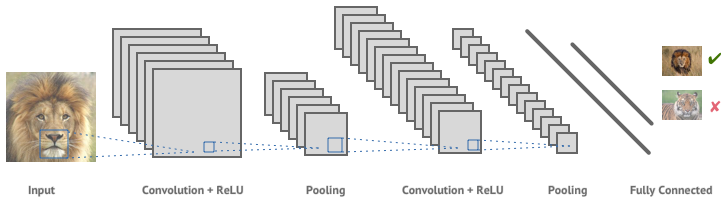
\includegraphics[scale=0.45]{conv.png}
\caption{exemplo de rede neural convolucional}
\label{fig:conv}
\end{figure}


Durante o treinamento de uma rede neural convolucional, os pesos são ajustados por meio de um algoritmo de otimização que minimiza uma função de perda. Entretanto, o ajuste dos pesos de uma rede neural convolucional é mais eficiente que o ajuste dos pesos de uma rede neural tradicional, pois, os pesos são compartilhados entre as camadas convolucionais, ou seja, os pesos são ajustados para todas as regiões da imagem. Por exemplo, considere uma imagem de $1000\times1000$ pixels e uma camada convolucional de $3\times3$ pixels, nesse caso, os pesos são ajustados para todas as regiões de $3\times3$ pixels da imagem. Sendo assim, o número de parâmetros que precisam ser ajustados é muito menor que o número de parâmetros de uma rede neural tradicional. Além disso, o cientista não precisa se preocupar em selecionar as características da imagem, pois, as camadas convolucionais são responsáveis por extrair as características da imagem automaticamente, os filtros possuem seus parâmetros ajustados durante o treinamento da rede neural, sendo que a única preocupação do cientista é definir a arquitetura da rede neural o que incluiu o número de camadas convolucionais e o número de filtros de cada camada convolucional.

Treinar uma rede neural convolucional do zero é um processo custoso, pois, é necessário um grande conjunto de dados para treinamento e um grande poder computacional para processar esses dados. Felizmente, após um modelo ser treinado, isto é, após encontrar os pesos ótimos de uma rede neural dado a função de erro e o conjunto de dados, é possível reutilizar esse modelo em outras aplicações, e, caso seja necessário, aplicar um pós-processamento para direcionar o modelo para uma aplicação específica. Sendo assim, foi encontrado na literatura um modelo de aprendizado profundo que já foi treinando para a tarefa de detecção de arestas, um dos modelos já estabelecidos para essa tarefa é o Holistically-Nested Edge Detection (HED) \cite{xie2015holisticallynested}. Esse modelo foi um aprimoramento da rede VGG-16 \cite{VGG16}, uma rede convolucional genérica que possuiu seus pesos treinados com milhões de imagens para Classificação, especializando-o para a detecção de arestas a partir do banco de dados BSDS500 \cite{BSDS500} que contém 500 imagens de treinamento e 200 imagens de teste que tiveram suas arestas selecionadas manualmente. Após o treinamento, o HED foi capaz de selecionar as arestas das imagens do banco de dados BSDS500 com uma acurácia de 0.790.

A vantagem do modelo HED em relação os modelos clássicos de detecção de arestas é que, por meio do aprendizado de máquina, ele consegue delimitar as bordas que compõem os objetos da imagem. Isso ocorre porque esse modelo conseguiu aprender as representações hierárquicas das imagens, ou seja, ele resolve o problema de ambiguidade entre a detecção de bordas e a segmentação de objetos. A figura \ref{fig:hed} mostra a fotografia do edifício da biblioteca nacional e o resultado da aplicação do modelo HED.

\begin{figure}[H]
\centering
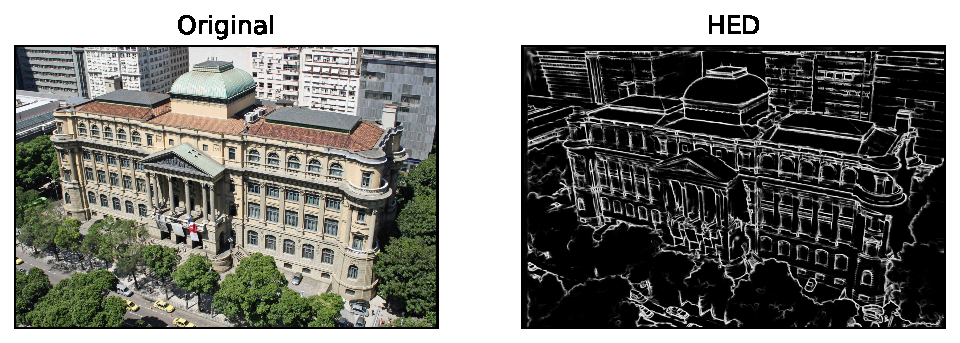
\includegraphics[scale=0.75]{bib_hed.pdf}
\caption{Imagem original e resultado do modelo HED.}
\label{fig:hed}
\end{figure}


\subsection{Resultados preliminares}

A seguir são apresentados os resultados comparativos da detecção de arestas utilizando o algoritmo de Canny e o modelo de aprendizado profundo pré-treinado HED. A figura \ref{fig:arestas} mostra a imagem original e o resultado da aplicação do algoritmo de Canny e do modelo HED. Observe que o modelo HED consegue selecionar as arestas que descreve melhor a forma dos edifícios, mas, distorce um pouco a forma das arestas. Por outro lado, o algoritmo de Canny não consegue selecionar as arestas que o descrevem melhor, mas, não distorce a forma das arestas. Para realizar o processamento foi utilizados a implementação dos modelos pela biblioteca \cite[Opencv]{opencv_library} na interface Python.


\begin{figure}[H]
\centering
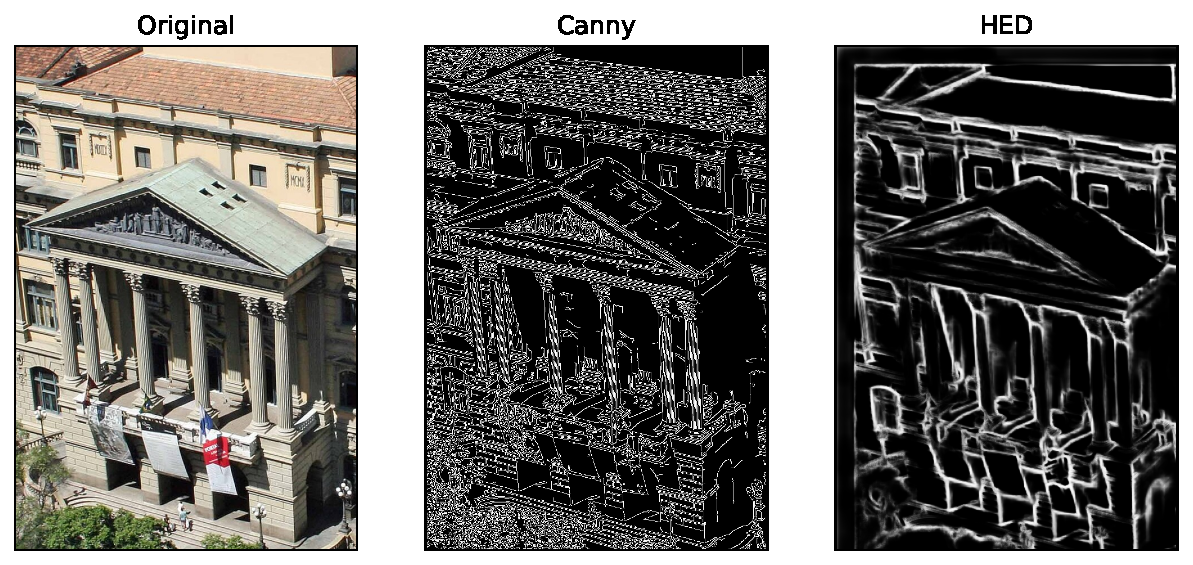
\includegraphics[scale=0.60]{bib_sub_filtro.pdf}
\caption{Imagem original e resultado da detecção de arestas.}
\label{fig:arestas}
\end{figure}

O modelo HED será utilizado no pipeline desse trabalho, e, a saída dessa etapa é uma imagem binária na qual cada pixel é classificado como aresta, pontos brancos, ou não, pontos pretos. A figura \ref{fig:bdarestas} mostra a imagem original e o resultado da aplicação do modelo HED na base de dados do ImageRio.

\begin{figure}
\centering
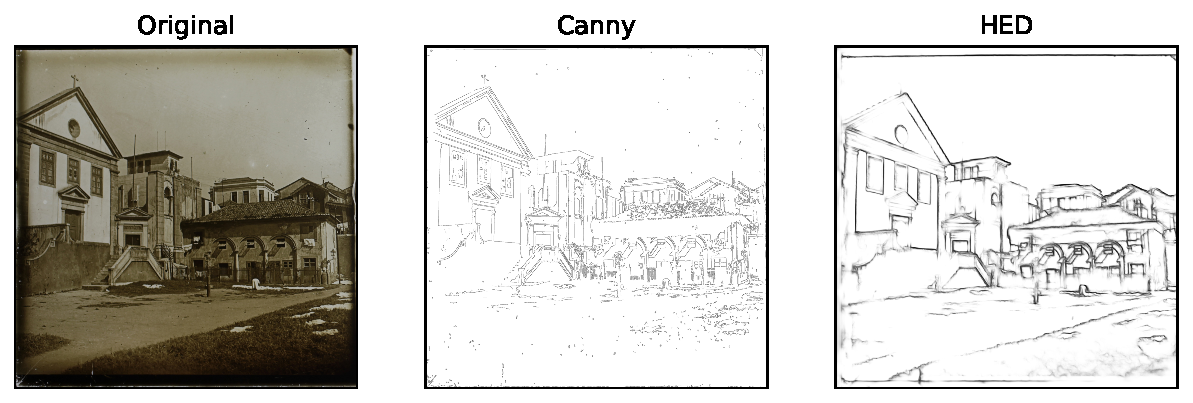
\includegraphics[scale=0.60]{exemple_edge.pdf}
\caption{Imagem original e resultado da detecção de arestas na base de dados do ImageRio.}
\label{fig:bdarestas}
\end{figure}

\section{Detecção de arestas}

O retorno da etapa anterior é uma imagem binária na qual cada pixel é classificado como aresta, pontos brancos, ou não, pontos pretos. Tradicionalmente, uma imagem representada como um conjunto de pontos num sistema de coordenadas cartesianas, onde cada ponto é representado por um pixel, possuiu a origem $(0,0)$ no ponto superior esquerdo da imagem e o eixo $x$ cresce para a direita e o eixo $y$ cresce para baixo. 

Sendo assim, o objetivo dessa etapa é identificar as equações dos segmentos de retas que compõem as arestas da imagem. Nesta etapa dois algoritmos foram testados: a transformada de Hough e a detecção de segmentos.

Antes de prosseguir pelo pipeline, foi observado que o modelo HED produz uma imagem com ruídos e que algumas arestas não são contínuas, ou seja, existem alguns pontos que não são conectados por uma aresta além de que existem arestas que são muito grossas o que pode gerar uma dupla detecção de arestas pelos algoritmos que se seguem. Para resolver esse problema, foi aplicado filtros morfológicos e filtros de suavização na imagem binária que serão discutidos na próxima subseção.

\subsection{filtros morfológicos}

Os filtros morfológicos \cite{HIPR2} são operadores que atuam em imagens binárias, ou seja, imagens que possuem apenas dois valores de intensidade, preto e branco. Esses filtros são baseados na teoria dos conjuntos e são utilizados para remover ruídos e para destacar as características de interesse da imagem. Os filtros morfológicos mais comuns são a erosão e a dilatação. A erosão remove os pixels brancos que estão próximos aos pixels pretos, ou seja, ela remove os pixels brancos que estão próximos as arestas. A dilatação adiciona pixels brancos próximos aos pixels brancos, ou seja, ela adiciona pixels brancos próximos as arestas. A abertura também é um filtro morfológico que é a composição da erosão com a dilatação, ou seja, a erosão é aplicada primeiro e depois a dilatação. A abertura remove os pixels brancos que estão próximos aos pixels pretos e adiciona pixels brancos próximos aos pixels brancos, ou seja, ela remove os pixels brancos que estão próximos as arestas e adiciona pixels brancos próximos as arestas. Outro filtro morfológico que foi utilizado foi o fechamento, que é a composição da erosão com a dilatação, ou seja, a erosão é aplicada primeiro e depois a dilatação. O fechamento remove os buracos dentro das arestas e preenche as arestas quebradas. A figura \ref{fig:morf} mostra a imagem original e o resultado da aplicação do fechamento e da erosão utilizado o opencv \cite{opencv_morphology} com um elemento estruturante de tamanho $(9\times9)$.

\begin{figure}
\centering
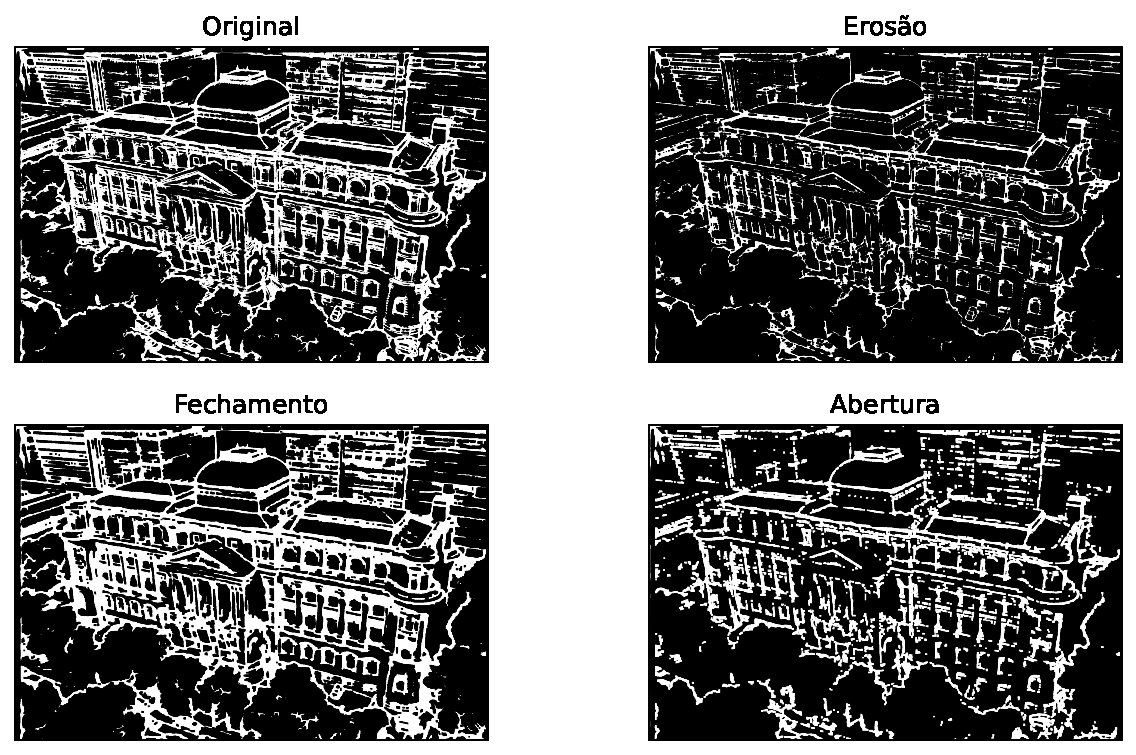
\includegraphics[scale=0.60]{morf.pdf}
\caption{Imagem original e resultado da aplicação dos filtros morfológicos.}
\label{fig:morf}
\end{figure}

É possível notar que o filtro de erosão consegue reduzir a espessura das arestas e o filtro de fechamento consegue remover os buracos dentro das arestas e preencher as arestas quebradas. Entretanto, o filtro de erosão ainda deixa arestas quebradiças e o filtro de fechamento ainda deixa arestas muito grossas. Para resolver o problema das arestas quebradiças, foi aplicado um filtro de suavização na imagem binária que será discutido na próxima subseção.

\subsection{Filtros de suavização}

Os filtros de suavização, também conhecidos como filtros de borramento, são operadores que amenizam as transições bruscas de intensidade da imagem. Neste caso, os filtros foram utilizados para suavizar as arestas quebradiças ao borrar a imagem. Os filtros de suavização que foram utilizados nesse trabalho foram o filtro de mediana e o filtro gaussiano. O filtro da mediana substitui o valor de um pixel pela mediana dos valores dos pixels vizinhos. O filtro gaussiano substitui o valor de um pixel pela média ponderada dos valores dos pixels vizinhos. A figura \ref{fig:blur} mostra a imagem original e o resultado da aplicação do filtro de mediana e do filtro gaussiano utilizado o opencv \cite{opencv_blur} com um kernel de tamanho $(5\times5)$.

\begin{figure}
\centering
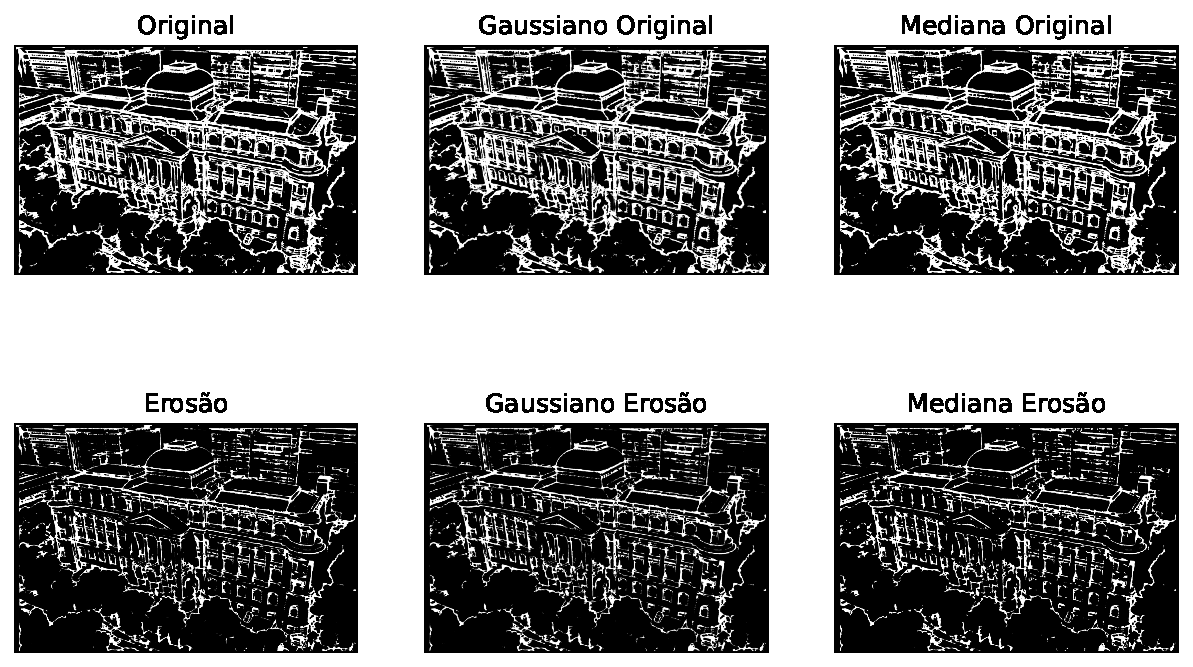
\includegraphics[scale=0.60]{blur.pdf}
\caption{Imagem original e resultado da aplicação dos filtros de suavização.}
\label{fig:blur}
\end{figure}



\subsection{Transformada de Hough}

A transformada de Hough \cite{illingworth1988survey} é um algoritmo de visão computacional que é capaz de detectar figuras geométricas em uma imagem, em especial retas. O algoritmo consiste em transformar a imagem de coordenadas cartesianas para coordenadas polares, onde cada ponto da imagem é representado por uma reta na imagem transformada. Nesse espaço, para encontrar uma reta, basta encontrar os pontos que se intersectam. Por isso, foi-se utilizado a transformada de Hough probabilística \cite{matas2000robust} que é uma versão mais eficiente da transformada de Hough. A figura \ref{fig:hough} mostra a imagem original e o resultado da aplicação da transformada de Hough probabilística utilizado o opencv \cite{opencv_hough}.


\begin{figure}
\centering
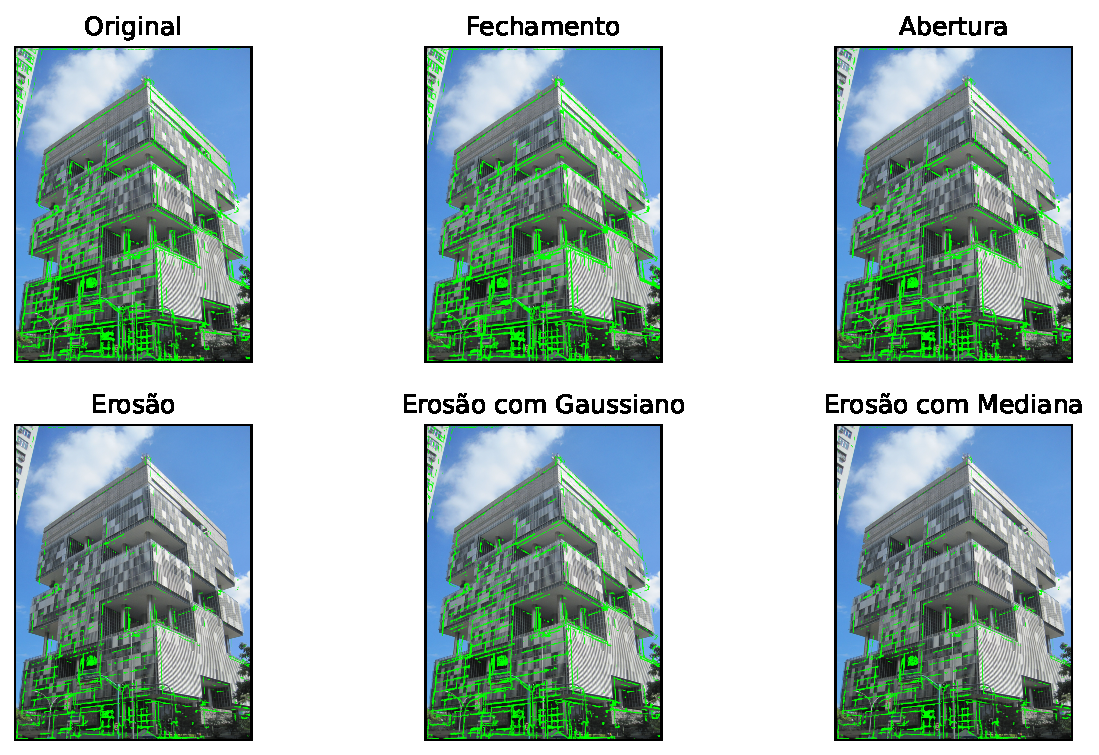
\includegraphics{houghP.pdf}
\caption{Imagem original e resultado da aplicação da transformada de Hough probabilística.}
\label{fig:hough}
\end{figure}

Nota-se que a transformada de Hough probabilística consegue detectar as arestas que compõem os edifícios, entretanto, ela não consegue detectar todas as arestas e algumas arestas são detectadas mais de uma vez. Por isso, foi testado um método mais robusto que será discutido na próxima subseção: a detecção de segmentos de retas.

\subsection{Detecção de segmentos a partir de pontos}

Para a detecção de segmentos, foi utilizada a implementação do Line Segment Detector \cite{opencv_manual} pela biblioteca opencv \cite{opencv_library} na interface Python. O LineSegmentDetector é um algoritmo de visão computacional que é capaz de detectar segmentos de retas em uma imagem, seu algoritmo é 


\subsection{Aprimoramento}

Observa-se que há muito ruído em alguns traços dos objetos selecionados pelo modelo de aprendizado de máquina, para evitar isso,  


\section{Classificação de segmentos}

A saída da etapa anterior $S$ contém o conjunto de pontos que descrevem os limites de segmentos de retas contidos na imagem



% \centering
% %left bottom right top
% %\includegraphics[trim=10mm 00mm 00mm 00mm, scale=0.40]{tabela.pdf}
% \begin{center}
% Figura 1: tabela.
% \end{center}

% \begin{figure}[H]
% \centering
% %left bottom right top
% %\includegraphics[trim=10mm 00mm 00mm 00mm, scale=0.40]{tabela.pdf}
% \begin{center}
% Figura 2: tabela.
% \end{center}
% \end{figure}

% \newpage
% \subsubsection{yy}

% yy

% % \[\left\{ 
% \begin{align*}
% f_{i}(x) = (10x + 100), \qquad \text{(1)} \tag{1}\\
% f_{ii}(x) = (20x + 200), \qquad \text{(2)} \tag{2} \\
% f_{iii}(x) = (30x + 300), \qquad \text{(3)} \tag{3} \\
% \end{align*} %\right.\]

% xx

% \begin{align*}
% Vm_{i}(p,l) = ((-1.9141)p + 49.466)l + ((199.51)p - 10795.0), \text {$l$=0} \tag{4}
% \end{align*}

% \begin{align*}
% f_{n}(y) = \frac{y}{1000}, \tag{5}
% \end{align*}

% \subsection{xx}

% xx

% %\[\left\{
% \begin{align*} 
% Funcao_{i}(p) = \gamma + \delta p + \theta p^2 + \omega p^3, \qquad \qquad \qquad \qquad \qquad \qquad \qquad \qquad \text{(6)} \tag{6} \\
% \end{align*} %\right.\]

% \newpage
% \section{Resultados Esperados}

% Nesta seção serão apresentados os resultados esperados...

% \subsection{xx}

% xx

\newpage
\section{Referências}

% [1] a.

% \noindent [2] b.

% \noindent [3] c.

% \noindent [4] d.

\printbibliography

\end{document}